% =================
% Bots
% =================
\subsection{Bot/Shell}
\label{sec:specie-bots}

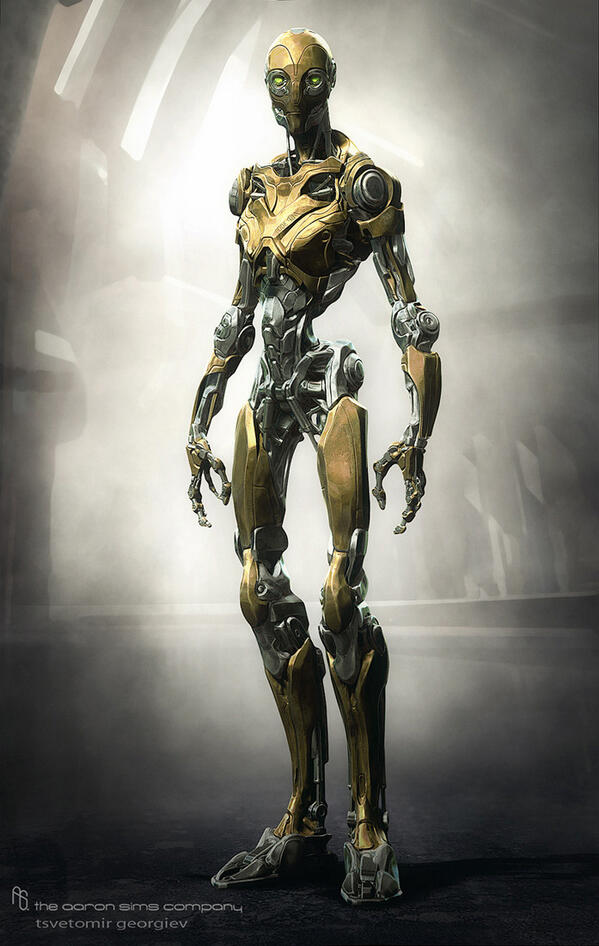
\includegraphics[width=\linewidth]{BEzZuPdCEAAgcr8}

A common sight on any technologically-advanced society is the large number of Bots and machines performing the menial yet necessary labour. Most of these machines are limited to a singular purpose and have a "weak AI". But technology has advanced far enough that some robots can be programmed to display human-like cognitive abilities. These Bots are called Artificial General Intelligences (AGI), and are used for highly specialised and complex work.

On the other end of the spectrum are individuals who have made the transition from organic to digital. These individuals, known as Ghosts, have chosen to digitise their conciousness and memory and upload themselves into artificial bodies known as Shells. Many in society believe that these digitised conciousnesses have lost their basic "humanity", and are indistinguishable from normal AI.

To create a Bot, Ghost or AGI character, please refer to the \textit{\hyperref[sec:rules-creation]{Character creation section}}

\textbf{Notes for AGI and Ghost characters:}

Your character will retain all of their memories and personality, and your Cortical Stack may be recoverable from the wreckage of your chassis (although all attributes, skills and edges will be lost with the chassis). If the Cortical Stack is damaged or lost, you can recover from a back-up (without all of the new memories). Purchasing new bodies is extremely expensive and your chassis model will only be able to improve a little bit before it hits it's technological limits.

It also should be noted that it is highly illegal to run multiple copies of yourself throughout the Federation and most Independent systems.

\begin{paperbox}{\textbf{Hacking}} 
Hacking a Bot is a very complex task. It will generally require the Hacker to access a physical I/O port, which is best accessed if the Bot is incapacitated. Then the Hacker needs to open the I/O port (Hacker's Repair vs Bot's Toughness), and then break the software Firewalls (Hacker's Security opposed by the Bot's Spirit).
\end{paperbox}

\begin{commentbox}{\textbf{Becoming the System}}
If you are a Ghost or AGI, there is nothing stopping you from inhabiting other digital systems. There are just a few cavaets:
  \begin{itemize}
    \item \textbf{Hardware}: Not all computer systems have the hardware needed to hold and operate a Ghost or AGI. In these cases it is better to interact with the system through a standard I/O port instead\\
    \item \textbf{Firewalls}: Unless you have been allowed to inhabit the system, there is likely to be multiple security systems in place to lock out and destroy intruders. Use the above Hacking rule\\
    \item \textbf{Limited Sensors}: Most systems do not even bother with audio visual input, relying on a user to type in commands through a terminal or keyboard. You could lose sense of the outside world while inhabiting the system\\
    \item \textbf{Illegal}: Across the Federation it is illegal for an AGI or Ghost to co-inhabit on a single computer with other AIs or programs. This is because most co-habited computers ended up with one "murdering" all other programs so that they can have uncontested access to system hardware. For this reason, all computer hardware must be blank before uploading an AGI or program, and (in the case of swapping) the hardware left behind must be blanked upon exiting\\
  \end{itemize}
\end{commentbox}
